\paragraph{QuizziPedia::Front-End::ModelViews::LoginModelView}
	
	\label{QuizziPedia::Front-End::ModelViews::LoginModelView}
	
	\begin{figure}[ht]
		\centering
		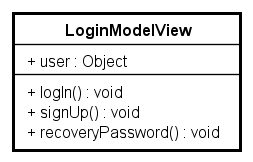
\includegraphics[scale=0.80,keepaspectratio]{UML/Classi/Front-End/QuizziPedia_Front-end_ModelView_LoginModelView.png}
		\caption{QuizziPedia::Front-End::ModelViews::LoginModelView}
	\end{figure} \FloatBarrier
	
	\begin{itemize}
		\item \textbf{Descrizione}: classe di tipo modelview la cui istanziazione è contenuta all'interno della variabile di ambiente \$scope di \textit{Angular.js\ped{G}}. All'interno di essa sono presenti le variabili e i metodi necessari per il \textit{Two-Way Data-Binding\ped{G}} tra la view \texttt{LoginView} e il controller \texttt{LoginController};
		\item \textbf{Utilizzo}: viene utilizzata per effettuare il \textit{Two-Way Data-Binding\ped{G}} tra la view \texttt{LoginView} e il controller \texttt{LoginController} rendendo disponibili variabili e metodi;
		\item \textbf{Relazioni con altre classi}: 
		\begin{itemize}
			\item \textit{OUT} \texttt{LoginView}: view contenente le form necessarie per effettuare il login. Contiene inoltre un link alla pagina di registrazione e uno alla pagina per il recupero della password; 
			\item \textit{OUT} \texttt{LoginController}: questa classe permette di gestire l'autenticazione dell'utente al sistema;
		\end{itemize}
		\item \textbf{Attributi}: 
		\begin{itemize}
				\item \texttt{+ user: Object} \\ Campo dati contenente due attributi: \texttt{username: String} e \texttt{password: String}.
		\end{itemize}
		\item \textbf{Metodi}: 
		\begin{itemize}
			\item \texttt{+} \texttt{logIn(): void} \\
			Metodo che richiama il metodo \texttt{Login} del service \texttt{AuthService} passandogli \texttt{username} e \texttt{password}. Nel caso di buona riuscita dell'operazione viene effettuato il redirect alla homepage dell'applicazione. Nel caso in cui invece avvenga un errore, viene mostrato a video il messaggio di errore;
			\item \texttt{+} \texttt{signUp(): void} \\
			Metodo che gestisce l’evento click sul pulsante di registrazione. Effettua il redirect alla pagina di registrazione;
			\item \texttt{+} \texttt{recoveryPassword(): void} \\
			Metodo che gestisce l’evento click sul pulsante di recupero password. Effettua il redirect alla pagina per il recupero della password; 
		\end{itemize}
	\end{itemize}
	
	